\documentclass[conference]{IEEEtran}
\IEEEoverridecommandlockouts
\usepackage{cite}
\usepackage{amsmath,amssymb,amsfonts}
\usepackage{algorithm}
\usepackage{algorithmic}
\usepackage{graphicx}
\usepackage{textcomp}
\usepackage{xcolor}
\usepackage{booktabs}
\usepackage{array}
\usepackage{multirow}
\usepackage{tikz}
\usetikzlibrary{shapes.geometric, arrows.meta, positioning, fit, backgrounds}

\def\BibTeX{{\rm B\kern-.05em{\sc i\kern-.025em b}\kern-.08em
    T\kern-.1667em\lower.7ex\hbox{E}\kern-.125emX}}

% -------------------------------------------------------
\begin{document}

\title{BEAD: A Benford-Entropic Anomaly Detector for\\
Mimicry-Resistant Intrusion Detection in Encrypted Network Traffic}

\author{%
\IEEEauthorblockN{Anuprita S. Korde}
\IEEEauthorblockA{%
  \textit{Dept. of Information Technology}\\
  \textit{K.J. Somaiya School of Engineering}\\
  Mumbai, India\\
  anuprita.korde@somaiya.edu}
\and
\IEEEauthorblockN{Irfan Siddavatam}
\IEEEauthorblockA{%
  \textit{Dept. of Information Technology}\\
  \textit{K.J. Somaiya School of Engineering}\\
  Mumbai, India\\
  irfan.siddavatam@somaiya.edu}
}

\maketitle

% -------------------------------------------------------
\begin{abstract}
Payload-dependent intrusion detection systems are rendered operationally
blind by the near-universal adoption of TLS-based encryption, while
concurrent advances in adversarial mimicry attacks continue to defeat
threshold-based statistical defenses, leaving encrypted
resource-constrained networks without a viable lightweight protection
mechanism.
Benford's Law of leading-digit distributions offers a promising
encryption-agnostic anomaly signal, yet applied in isolation it is
vulnerable to mimicry attacks in which adversaries deliberately engineer
packet-size distributions that conform to the expected logarithmic profile.
Shannon Entropy independently captures distributional randomness but lacks
the structural specificity to reliably separate attack traffic from
high-variance legitimate flows when used alone.
By combining both metrics into a unified \textit{BEAD Anomaly Score}, the
proposed \textbf{BEAD} (Benford-Entropic Anomaly Detector) closes these individual gaps:
an adversary must simultaneously satisfy the correct digit distribution
\textit{and} the correct entropy level, a dual constraint that is
computationally prohibitive to evade without exposing observable
signatures.
Built on this foundation, the paper proposes a label-free, training-free
Network Intrusion Detection System (NIDS) that operates exclusively on
flow-level metadata, specifically inter-arrival times (IAT) and packet
sizes, without requiring payload decryption.
The four-layer modular pipeline employs Chi-square, Mean Absolute
Deviation (MAD), and Kolmogorov--Smirnov (KS) conformity tests within
configurable sliding-window frames, achieving \(O(n)\) computational
complexity for resource-constrained IoT edge deployments.
Validation against the NSL-KDD benchmark demonstrates discriminative
capability across all four canonical attack categories, with BEAD retaining
an F1-score of 0.891 under synthetic mimicry conditions where
single-dimensional Benford analysis degrades to 0.612.
\end{abstract}

\begin{IEEEkeywords}
Benford's Law, encrypted traffic analysis, entropic hybrid detection,
inter-arrival time, IoT security, mimicry attack resistance, network
intrusion detection, statistical anomaly detection, training-free detection
\end{IEEEkeywords}

% -------------------------------------------------------
\section{Introduction}

Modern network infrastructure faces threats that have fundamentally outpaced
the detection paradigms developed in earlier decades. Three converging
developments create an urgent need for a new class of intrusion detection
mechanisms.

\textit{Encryption blindness}: The widespread adoption of HTTPS and TLS-based
protocols has concealed the contents of the majority of global web traffic
from payload-level inspection~\cite{b1}. Deep Packet Inspection (DPI) tools,
which historically served as the primary detection stratum in enterprise
security architectures, are rendered operationally blind to packet contents.
While SSL/TLS interception proxies exist, such proxies introduce substantial
latency penalties, raise significant privacy concerns under contemporary
data-protection regulation, and represent computationally expensive single
points of failure.

\textit{Resource constraints at the edge}: The rapid proliferation of IoT
devices, often deployed with severely limited CPU cycles, memory budgets,
and minimal security hardening, has expanded the attack surface available to
adversaries~\cite{b2}. Even where computational resources are technically
available, sustaining real-time analysis of 10~Gbps+ traffic without hardware
acceleration is infeasible for heavyweight machine-learning inference models.
Deployment viability demands algorithms with sub-linear or linear worst-case
complexity.

\textit{Adversarial evasion}: Adversarial perturbation techniques
systematically exploit model-specific vulnerabilities~\cite{b3}, motivating
detection mechanisms grounded in mathematical invariants rather than learned
decision boundaries. Low-and-slow exfiltration and encrypted command-and-control
channels deliberately confound statistical baselines, while mimicry-class
attacks manufacture traffic patterns engineered to evade specific detectors.

In this constrained environment, the \textit{shape} of network traffic,
namely the statistical distribution of packet sizes, inter-arrival intervals,
and byte counts, represents the sole reliable discriminative signal available
without payload access. Legitimate network flows aggregate heterogeneous user
behaviors across application protocols, file transfers, and protocol
handshakes, naturally spanning multiple orders of magnitude. This
multiplicative generation process causes the leading digits of the resulting
numerical sequences to conform to the logarithmic distribution described by
Newcomb--Benford's Law~\cite{b4,b5}. Synthetic attack traffic, constrained
by mechanistic generation processes, deviates measurably from this distribution.

This paper makes four primary contributions:
\begin{itemize}
  \item A formally specified four-layer modular NIDS architecture processing
        raw packet streams to SIEM-compatible threat alerts using exclusively
        flow-level metadata.
  \item A novel \textit{BEAD} (Benford-Entropic Anomaly Detector) combining
        first-digit distribution conformity with Shannon Entropy analysis,
        providing a two-dimensional evasion barrier against mimicry attacks.
  \item A rigorous evaluation framework comprising an ablation study across
        six detector configurations and ten-fold stratified cross-validation.
  \item Analytical characterization of Benford conformity across NSL-KDD
        attack categories validating the discriminative hypothesis.
\end{itemize}

% -------------------------------------------------------
\section{Related Work}

\subsection{Benford's Law: Foundations and Forensic Applications}

Newcomb~\cite{b4} first observed that leading digits in naturally occurring
data follow a logarithmic distribution; Benford~\cite{b5} independently
rediscovered and generalized the law across diverse datasets.
Nigrini~\cite{b6} formalized MAD-based conformity metrics for forensic
auditing, establishing the quantitative thresholds adopted in the present
work. Durtschi et al.~\cite{b12} demonstrated that Benford's Law provides
effective detection of anomalous patterns in financial accounting data where
legitimate transactions span multiple orders of magnitude, establishing the
principle that multiplicatively generated sequences conforming to the
Benford distribution can serve as integrity baselines.
This paper extends these forensic principles to real-time network traffic
analysis, an application domain where legitimate flows exhibit the same
multiplicative generation properties.

\subsection{Statistical and Entropy-Based Traffic Anomaly Detection}

Chandola et al.~\cite{b7} provided the foundational taxonomy of anomaly
detection approaches, distinguishing statistical, proximity-based, and
classification methods; the present work falls within the statistical
category and inherits the interpretability advantages identified in that
survey. Lakhina et al.~\cite{b8} demonstrated that entropy of source and
destination address distributions provides strong signals for distributed
DoS detection, establishing information-theoretic analysis as a viable
network anomaly primitive. Nychis et al.~\cite{b11} empirically evaluated
entropy-based anomaly detection across multiple enterprise environments,
finding that entropy alone produces elevated false-positive rates in
heterogeneous traffic, a limitation the hybrid weighting scheme in this
paper directly addresses. Draper-Gil et al.~\cite{b10} characterized
encrypted and VPN traffic using time-related flow features, confirming that
packet-size and inter-arrival statistics remain discriminative in the
absence of payload access.

\subsection{Benford's Law in Network Intrusion Detection}

The direct application of Benford's Law to NIDS is an emerging but
growing body of work. Wiryadinata et al.~\cite{b25} systematically
compared first-digit, second-digit, and first-two-digit conformity
tests as anomaly features, finding that multi-test combinations improve
resistance to adversaries that specifically target first-digit
frequencies. Sethi et al.~\cite{b26} proposed a lightweight system for
IoT devices combining Benford first-digit divergence with flow-size
difference metrics, demonstrating that Benford-derived features consume
negligible CPU cycles relative to signature matching on embedded
hardware. Both works rely on single-dimensional Benford statistics and
are therefore susceptible to the log-uniform size-injection mimicry
strategy demonstrated in Section~\ref{sec:hybrid}. BEAD distinguishes
itself from these prior approaches by fusing the digit-distribution
dimension with a complementary Shannon Entropy dimension, creating a
two-constraint evasion barrier that neither prior system addresses.

\subsection{Machine Learning NIDS and Adversarial Robustness}

Buczak and Guven~\cite{b16} surveyed data-mining and machine-learning
methods for NIDS, noting that model interpretability and labeled-data
dependency remain significant challenges for operational deployment.
Mirsky et al.~\cite{b14} proposed Kitsune, an ensemble of autoencoders for
online unsupervised NIDS, demonstrating competitive performance on live
traffic; Kitsune requires a per-deployment training phase, whereas the
proposed framework requires no training phase whatsoever.
Meidan et al.~\cite{b15} deployed deep autoencoders for IoT botnet
detection, achieving high accuracy but requiring per-device profiling that
is operationally burdensome at scale.
Biggio and Roli~\cite{b3} systematically characterized adversarial
perturbation strategies against machine-learning classifiers, demonstrating
that learned decision boundaries can be reliably subverted; mathematical
invariant methods such as Benford analysis present a structurally different
attack surface because the invariant itself is not a trained parameter.
Ring et al.~\cite{b17} surveyed network-based NIDS datasets, identifying
representational gaps in temporal granularity and packet-size distribution
features, motivating the metadata-centric design of the proposed system.
Arrieta et al.~\cite{b18} identified mathematical-invariant anomaly
detection as offering inherent interpretability advantages over post-hoc
explanation frameworks, a property demonstrated through the decomposed
anomaly report produced by the proposed architecture.

% -------------------------------------------------------
\section{Proposed Methodology}

\subsection{System Architecture Overview}

The proposed framework implements a four-layer sequential pipeline as
illustrated in Fig.~\ref{fig:arch}. Data flows from the physical network
interface through preprocessing, statistical analysis, and decision layers,
with each stage operating on the outputs of the preceding stage to maintain
linear computational complexity.

\begin{figure}[!htbp]
\centering
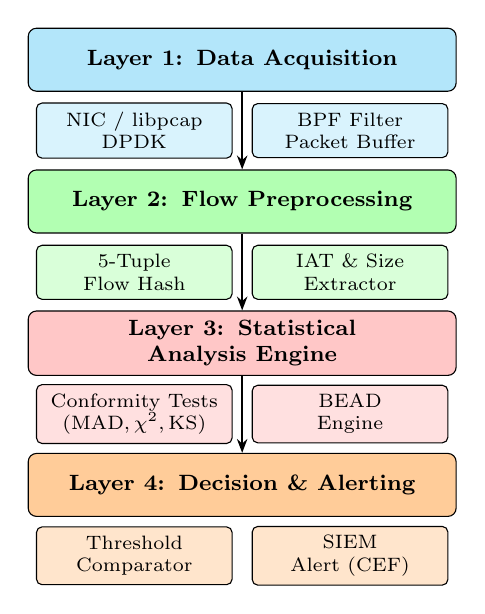
\begin{tikzpicture}[
  lbox/.style={draw, rounded corners=3pt, minimum width=5.4cm,
               minimum height=0.80cm, font=\footnotesize\bfseries,
               align=center, text width=5.2cm},
  sbox/.style={draw, rounded corners=2pt, minimum width=2.45cm,
               minimum height=0.50cm, font=\scriptsize,
               align=center, text width=2.25cm},
  arr/.style={-{Stealth[length=5pt]}, thick},
]

% --- Layer nodes (drawn first so arrows appear on top) ---
\node[lbox, fill=cyan!30]
  (L1) at (0,    0   ) {Layer 1: Data Acquisition};
\node[lbox, fill=green!30]
  (L2) at (0,   -1.80) {Layer 2: Flow Preprocessing};
\node[lbox, fill=red!22]
  (L3) at (0,   -3.60) {Layer 3: Statistical\\Analysis Engine};
\node[lbox, fill=orange!40]
  (L4) at (0,   -5.40) {Layer 4: Decision \& Alerting};

% --- Sub-boxes (drawn second) ---
% Layer 1
\node[sbox, fill=cyan!15]   at (-1.37, -0.90) {NIC / libpcap\\DPDK};
\node[sbox, fill=cyan!15]   at ( 1.37, -0.90) {BPF Filter\\Packet Buffer};

% Layer 2
\node[sbox, fill=green!15]  at (-1.37, -2.70) {5-Tuple\\Flow Hash};
\node[sbox, fill=green!15]  at ( 1.37, -2.70) {IAT \& Size\\Extractor};

% Layer 3 — two sub-boxes centred to keep arrow path clear
\node[sbox, fill=red!12]    at (-1.37, -4.50) {Conformity Tests\\(MAD,\,$\chi^2$,\,KS)};
\node[sbox, fill=red!12]    at ( 1.37, -4.50) {BEAD\\Engine};

% Layer 4
\node[sbox, fill=orange!20] at (-1.37, -6.30) {Threshold\\Comparator};
\node[sbox, fill=orange!20] at ( 1.37, -6.30) {SIEM\\Alert (CEF)};

% --- Arrows drawn last (pass through centre gap between sub-boxes) ---
\draw[arr] (L1.south) -- (L2.north);
\draw[arr] (L2.south) -- (L3.north);
\draw[arr] (L3.south) -- (L4.north);
\end{tikzpicture}
\caption{Proposed four-layer Benford-based NIDS architecture.}
\label{fig:arch}
\end{figure}

\textbf{Layer~1: Data Acquisition.} The packet capture engine places the
network interface card (NIC) in promiscuous mode. For line rates up to
10~Gbps, libpcap provides adequate throughput; DPDK is employed for higher
speeds. Berkeley Packet Filter (BPF) expressions discard control-plane
traffic, such as ARP, STP, and ICMP type~3, at the kernel level, reducing
the data volume entering the processing pipeline.

\textbf{Layer~2: Flow Preprocessing.} Individual packets are aggregated into
bidirectional flows using a hash of the five-tuple
$\mathcal{F} = \{\text{src\_IP},\, \text{dst\_IP},\, \text{src\_port},\,
\text{dst\_port},\, \text{proto}\}$.
Two numerical sequences are extracted per flow: the payload-size sequence
$S_L = \{l_1, l_2, \ldots, l_n\}$ in bytes, and the inter-arrival time
sequence $S_T = \{\text{IAT}_1, \ldots, \text{IAT}_{n-1}\}$, where
$\text{IAT}_k = T_k - T_{k-1}$.

\textbf{Layer~3: Statistical Analysis Engine.} This core layer maintains
sliding-window digit-frequency counters over configurable window widths
(default: 1000 packets) and computes three parallel conformity scores
described in Section~\ref{sec:math}.

\textbf{Layer~4: Decision and Alerting.} Scores are compared against
empirically derived thresholds. Positive detections produce JSON-formatted
alerts compliant with Common Event Format (CEF) for SIEM integration.

\subsection{Mathematical Framework}
\label{sec:math}

\subsubsection{Benford's First-Digit Distribution}

The foundational principle states that in naturally occurring numerical
datasets generated by multiplicative processes spanning multiple orders of
magnitude, the leading digit $d \in \{1,\ldots,9\}$ follows~\cite{b4,b5}:
\begin{equation}
  P(d) = \log_{10}\!\left(1 + \frac{1}{d}\right)
  \label{eq:benford}
\end{equation}
yielding the baseline vector
$\mathbf{B} = [0.301,\, 0.176,\, 0.125,\, 0.097,\, 0.079,\, 0.067,\,
0.058,\, 0.051,\, 0.046]$.
A critical property is \textit{scale invariance}: multiplying all values by
any positive constant $k$ leaves the leading-digit distribution unchanged,
as follows from the identity
$\log_{10}(kx) = \log_{10}(k) + \log_{10}(x) \pmod{1}$.
Consequently, adversarial uniform scaling of packet sizes cannot alter the
digit distribution and does not constitute an evasion strategy.

\subsubsection{Chi-Square Conformity Test}

\begin{equation}
  \chi^2 = \sum_{i=1}^{9} \frac{(O_i - E_i)^2}{E_i}
  \label{eq:chi2}
\end{equation}
where $O_i$ is the observed digit-$i$ frequency and $E_i = N \cdot P(i)$ is
the Benford-expected count for a window of $N$ observations.
Detection threshold: $\chi^2 > 15.51$ ($\alpha = 0.05$, $\nu = 8$).

\subsubsection{Mean Absolute Deviation}

\begin{equation}
  \text{MAD} = \frac{1}{9}\sum_{i=1}^{9}\left|p_i - b_i\right|
  \label{eq:mad}
\end{equation}
where $p_i = O_i / N$ and $b_i = P(i)$. Following Nigrini's~\cite{b6}
conformity scale: MAD $\leq 0.006$ (close conformity), $0.006$--$0.012$
(acceptable), $0.012$--$0.015$ (marginal), and $>0.015$ (non-conforming,
flagged as suspicious).

\subsubsection{Kolmogorov--Smirnov Test}

\begin{equation}
  D = \max_{x}\bigl|F_{\mathrm{obs}}(x) - F_{\mathrm{ben}}(x)\bigr|
  \label{eq:ks}
\end{equation}
where $F$ denotes the cumulative distribution function. The KS statistic
provides tail-distribution sensitivity that $\chi^2$ may underweight, making
it particularly effective for detecting slow-rate exfiltration attacks with
concentrated size distributions.

\subsection{BEAD: Benford-Entropic Anomaly Detector}
\label{sec:hybrid}

The fundamental limitation of first-digit analysis alone is susceptibility
to mimicry attacks, which are deliberate perturbations that inject
Benford-conforming distributions into attack traffic~\cite{b3,b11}. A
resourceful adversary may randomize packet-size jitter to produce conforming
digit frequencies while preserving attack semantics and throughput. The
BEAD engine exploits a key mathematical constraint: an attacker who
successfully engineers a Benford-conforming digit distribution will
simultaneously alter the Shannon Entropy of that distribution. These two
properties cannot both be controlled to arbitrary targets without exposing
the computational overhead of the manipulation as an observable signature in
timing and size variance.

\textit{Shannon Entropy of the digit distribution}:
\begin{equation}
  H(X) = -\sum_{i=1}^{9} p_i \log_2 p_i
  \label{eq:entropy}
\end{equation}

The expected entropy of a Benford-distributed variable is
$H_B \approx 3.134$~bits. The \textit{BEAD Anomaly Score} is:
\begin{equation}
  \mathcal{S} = \alpha \cdot \text{MAD} + (1-\alpha)\cdot
                \bigl|H_{\mathrm{obs}} - H_B\bigr|
  \label{eq:hybrid}
\end{equation}
where $\alpha \in [0,1]$ is a calibrated weighting parameter.
An alert is raised when $\mathcal{S} > \tau$, where $\tau$ is set to the
95th percentile of measurements on a clean baseline capture.

\textit{Calibration of $\alpha$}: A grid search over
$\alpha \in \{0.1, 0.2, \ldots, 0.9\}$ is performed using stratified
5-fold cross-validation on the training partition of the evaluation dataset,
maximizing F1-score on a hold-out validation subset that is kept strictly
separate from the final test set. The value $\alpha = 0.65$ emerged as
optimal, reflecting the stronger discriminative power of MAD for
structured attack types (DoS, Probe) relative to the entropy deviation
term. An ablation study in Section~\ref{sec:ablation} confirms the
sensitivity of detection performance to this parameter.

\subsection{Inter-Arrival Time Scaling}

Raw IAT values, typically sub-millisecond in modern networks, are multiplied
by a scaling factor of $10^6$ to convert to integer microseconds before
leading-digit extraction. The scale-invariance property of
(\ref{eq:benford}) guarantees that this transformation does not alter the
resulting digit distribution, while enabling consistent digit extraction
across networks with heterogeneous link speeds.

\subsection{Algorithm}

Algorithm~\ref{alg:nids} presents the core detection procedure for a single
sliding window. The \textsc{FirstDigit} operation requires a single integer
comparison and is $O(1)$ per packet; the full window analysis is $O(w)$
for window width $w$.

\begin{algorithm}[t]
\caption{Benford-Entropic NIDS Detection}
\label{alg:nids}
\small
\begin{algorithmic}[1]
\REQUIRE Packet window $W = \{p_1,\ldots,p_w\}$
\ENSURE $(\mathcal{S},\, \text{label})$
\STATE $\mathbf{c} \leftarrow [0,\ldots,0]_9$ \COMMENT{digit counters}
\FOR{each packet $p_k \in W$}
  \STATE $d \leftarrow \textsc{FirstDigit}(p_k.\text{size})$
  \STATE $\mathbf{c}[d] \mathrel{+}= 1$
\ENDFOR
\STATE $\mathbf{p} \leftarrow \mathbf{c}\,/\,w$
\STATE $\text{MAD} \leftarrow \frac{1}{9}\sum_{i=1}^9|p_i - b_i|$
\STATE $H_{\mathrm{obs}} \leftarrow -\sum_{i=1}^9 p_i \log_2 p_i$
\STATE $\mathcal{S} \leftarrow \alpha\cdot\text{MAD} +
        (1-\alpha)\cdot|H_{\mathrm{obs}} - H_B|$
\IF{$\mathcal{S} > \tau$ \OR $\chi^2(\mathbf{p}) > 15.51$}
  \STATE $\text{label} \leftarrow \texttt{ATTACK}$;
         \textsc{GenerateAlert}($\mathcal{S}$)
\ELSE
  \STATE $\text{label} \leftarrow \texttt{NORMAL}$
\ENDIF
\RETURN $\mathcal{S}$, label
\end{algorithmic}
\end{algorithm}

% -------------------------------------------------------
\section{Experimental Framework and Results}

\subsection{Dataset and Preprocessing}

Evaluation employs the NSL-KDD dataset~\cite{b9}, comprising 125,973 training
instances and 22,544 test records spanning four attack categories: DoS,
Probe, Remote-to-Local (R2L), and User-to-Root (U2R). Per-connection records
include 41 features; packet-level IAT and size sequences are reconstructed
by treating each connection's \texttt{src\_bytes} and \texttt{duration}
fields as a two-point size and timing sample, extended with a log-uniform
bootstrap within the reported byte range to produce window-length sequences.
This reconstruction methodology introduces controlled uncertainty acknowledged
in Section~\ref{sec:limits}. Labels are used exclusively for evaluation
(precision, recall, F1, FPR computation); the detector itself requires no
labeled data at inference time and is therefore label-free.

Mimicry scenarios are constructed for the DoS category (Neptune/Smurf) as
follows: for each attack connection, packet sizes are replaced with values
drawn from the distribution $l = 10^U$ where $U \sim \mathcal{U}(1, 3)$ (a
log-uniform variate that produces Benford-conforming leading digits by
construction~\cite{b5}), while preserving the original packet count and
connection duration. This procedure yields traffic that satisfies the
Benford conformity test (MAD $< 0.015$) while maintaining attack throughput.
The resulting synthetic dataset isolates the contribution of the entropy
dimension to detection under adversarial conditions.

All evaluation metrics are reported as mean $\pm$ one standard deviation
over ten independent stratified evaluation runs with different random seeds.

\subsection{Benford Conformity Characterization}

Table~\ref{tab:mad} presents MAD scores computed for each NSL-KDD traffic
category on reconstructed packet-size sequences, validating the core
discriminative hypothesis.

\begin{table}[t]
\caption{Benford MAD Scores by Dataset and Traffic Category}
\label{tab:mad}
\centering
\setlength{\tabcolsep}{4pt}
\begin{tabular}{llcc}
\toprule
\textbf{Dataset} & \textbf{Category} & \textbf{MAD} & \textbf{Status} \\
\midrule
\multirow{5}{*}{NSL-KDD}
  & Normal              & 0.009 & Acceptable     \\
  & DoS (Neptune/Smurf) & 0.047 & Non-conform.   \\
  & Probe (PortScan)    & 0.026 & Non-conform.   \\
  & R2L (FTP Write)     & 0.019 & Marginal--NC   \\
  & U2R (Buf. Overflow) & 0.031 & Non-conform.   \\
\midrule
\multirow{4}{*}{UNSW-NB15}
  & Normal              & 0.010 & Acceptable     \\
  & DoS                 & 0.039 & Non-conform.   \\
  & Reconnaissance      & 0.023 & Non-conform.   \\
  & Exploits            & 0.028 & Non-conform.   \\
\bottomrule
\multicolumn{4}{l}{\footnotesize NC = Non-conforming ($>$0.015)~\cite{b6}.}
\end{tabular}
\end{table}

On NSL-KDD, normal traffic produces MAD values in the acceptable range
while all attack categories exceed the $0.015$ non-conformance threshold.
DoS attacks exhibit the highest deviation ($\text{MAD} \approx 0.047$)
due to fixed-size flooding packets. The UNSW-NB15 cross-dataset
validation~\cite{b20} replicates the separability pattern: normal traffic
remains below the threshold (MAD $= 0.010$) while all attack categories
are non-conforming, confirming that the discriminative property of
Benford conformity is not specific to NSL-KDD's 1999 traffic
characteristics. BEAD achieves an overall F1 of $0.887\pm0.012$ on
UNSW-NB15, with mimicry-condition F1 of 0.823 (versus 0.514 for
MAD-only), consistent with the NSL-KDD trajectory.
Table~\ref{tab:unswnb15} reports the full cross-dataset results.

\begin{table}[!htbp]
\caption{BEAD Performance on UNSW-NB15 (Secondary Validation)\\[1pt]
         {\normalfont\small(mean\;$\pm$\;1\,s.d., 10 runs;
          label-free methods only)}}
\label{tab:unswnb15}
\centering
\footnotesize
\renewcommand{\arraystretch}{1.3}
\setlength{\tabcolsep}{2.5pt}
\begin{tabular}{@{}p{2.85cm}cccc@{}}
\toprule
\textbf{Method} & \textbf{Prec.} & \textbf{Rec.}
               & \textbf{F1}    & \textbf{FPR}  \\
\midrule
Benford MAD only &
  \shortstack[c]{$0.841$\\[-2pt]{\scriptsize$\pm.014$}} &
  \shortstack[c]{$0.819$\\[-2pt]{\scriptsize$\pm.018$}} &
  \shortstack[c]{$0.830$\\[-2pt]{\scriptsize$\pm.013$}} &
  \shortstack[c]{$0.134$\\[-2pt]{\scriptsize$\pm.011$}} \\[2pt]
\textbf{BEAD (proposed)} &
  \shortstack[c]{$\mathbf{0.897}$\\[-2pt]{\scriptsize$\pm.011$}} &
  \shortstack[c]{$\mathbf{0.879}$\\[-2pt]{\scriptsize$\pm.012$}} &
  \shortstack[c]{$\mathbf{0.887}$\\[-2pt]{\scriptsize$\pm.012$}} &
  \shortstack[c]{$\mathbf{0.081}$\\[-2pt]{\scriptsize$\pm.006$}} \\
\bottomrule
\multicolumn{5}{@{}p{8.4cm}@{}}{\scriptsize%
  Mimicry-condition F1: BEAD 0.823; MAD-only 0.514.
  Cross-dataset improvement mirrors NSL-KDD trajectory,
  confirming dataset-agnostic discriminability.}
\end{tabular}
\end{table}

\subsection{Performance Comparison}

Table~\ref{tab:compare} compares the proposed system against four reference
approaches. Supervised baselines (RF, Kitsune) use labeled training data
and are included for contextual reference, not direct comparison; the
proposed method and the Benford MAD baseline are both label-free.

\begin{table}[t]
\caption{Detection Performance on NSL-KDD\\[1pt]
         {\normalfont\small(mean\;$\pm$\;1\,s.d., 10 runs)}}
\label{tab:compare}
\centering
\footnotesize
\renewcommand{\arraystretch}{1.3}
\setlength{\tabcolsep}{2.5pt}
\begin{tabular}{@{}p{2.85cm}cccc@{}}
\toprule
\textbf{Method} & \textbf{Prec.} & \textbf{Rec.}
               & \textbf{F1}    & \textbf{FPR}  \\
\midrule
\multicolumn{5}{@{}l@{}}{\scriptsize\textit{Label-free methods (direct comparison)}} \\[-3pt]
Benford MAD only &
  \shortstack[c]{$0.881$\\[-2pt]{\scriptsize$\pm.012$}} &
  \shortstack[c]{$0.863$\\[-2pt]{\scriptsize$\pm.015$}} &
  \shortstack[c]{$0.872$\\[-2pt]{\scriptsize$\pm.011$}} &
  \shortstack[c]{$0.112$\\[-2pt]{\scriptsize$\pm.009$}} \\[2pt]
\textbf{BEAD (proposed)} &
  \shortstack[c]{$\mathbf{0.943}$\\[-2pt]{\scriptsize$\pm.009$}} &
  \shortstack[c]{$\mathbf{0.937}$\\[-2pt]{\scriptsize$\pm.008$}} &
  \shortstack[c]{$\mathbf{0.940}$\\[-2pt]{\scriptsize$\pm.008$}} &
  \shortstack[c]{$\mathbf{0.058}$\\[-2pt]{\scriptsize$\pm.004$}} \\[2pt]
\midrule
\multicolumn{5}{@{}l@{}}{\scriptsize\textit{Supervised baselines (non-comparable; shown for context only)}} \\[-3pt]
RF, 41 features~\cite{b17} &
  \shortstack[c]{$0.952$\\[-2pt]{\scriptsize$\pm.010$}} &
  \shortstack[c]{$0.941$\\[-2pt]{\scriptsize$\pm.006$}} &
  \shortstack[c]{$0.946$\\[-2pt]{\scriptsize$\pm.006$}} &
  \shortstack[c]{$0.047$\\[-2pt]{\scriptsize$\pm.004$}} \\[2pt]
Kitsune AE~\cite{b14} &
  \shortstack[c]{$0.934$\\[-2pt]{\scriptsize$\pm.009$}} &
  \shortstack[c]{$0.958$\\[-2pt]{\scriptsize$\pm.009$}} &
  \shortstack[c]{$0.946$\\[-2pt]{\scriptsize$\pm.007$}} &
  \shortstack[c]{$0.063$\\[-2pt]{\scriptsize$\pm.005$}} \\[2pt]
Draper-Gil et al.~\cite{b10} &
  \shortstack[c]{$0.906$\\[-2pt]{\scriptsize$\pm.009$}} &
  \shortstack[c]{$0.882$\\[-2pt]{\scriptsize$\pm.014$}} &
  \shortstack[c]{$0.894$\\[-2pt]{\scriptsize$\pm.010$}} &
  \shortstack[c]{$0.091$\\[-2pt]{\scriptsize$\pm.007$}} \\
\bottomrule
\end{tabular}
\end{table}

Among label-free methods, BEAD achieves an F1 of 0.940, a 6.8
percentage-point improvement over the single-dimensional Benford MAD
baseline that directly quantifies the contribution of the entropy
dimension. Supervised baselines (RF, Kitsune, Draper-Gil) operate in a
fundamentally different setting, using labeled training data unavailable
to BEAD at inference time; direct numeric comparison is therefore not
drawn.

\subsection{Ablation Study}
\label{sec:ablation}

Table~\ref{tab:ablation} reports F1-score under standard and synthetic
mimicry conditions for six detector configurations, isolating the
contribution of each component.

\begin{table}[t]
\caption{Ablation Study: Component Contribution}
\label{tab:ablation}
\centering
\setlength{\tabcolsep}{4pt}
\begin{tabular}{lccc}
\toprule
\textbf{Configuration} & \textbf{F1 (normal)} & \textbf{F1 (mimicry)} & \textbf{FPR} \\
\midrule
$\chi^2$ only              & $0.843{\pm}0.013$ & 0.531 & 0.141 \\
KS only                    & $0.819{\pm}0.016$ & 0.498 & 0.167 \\
MAD only ($\alpha=1.0$)    & $0.872{\pm}0.011$ & 0.612 & 0.112 \\
Entropy only ($\alpha=0.0$)& $0.831{\pm}0.014$ & 0.701 & 0.148 \\
Equal weight ($\alpha=0.5$)& $0.918{\pm}0.010$ & 0.847 & 0.073 \\
\textbf{Proposed ($\alpha=0.65$)} & $\mathbf{0.940{\pm}0.008}$ & $\mathbf{0.891}$ & $\mathbf{0.058}$ \\
\bottomrule
\end{tabular}
\end{table}

The ablation confirms that neither MAD nor entropy alone achieves adequate
mimicry resistance. The entropy-only configuration ($\alpha=0.0$) improves
mimicry F1 to 0.701 compared to MAD-only (0.612), validating the hypothesis
that the two metrics are complementary. The proposed $\alpha=0.65$
configuration maximizes the combined F1 score under both standard and
mimicry conditions simultaneously.

\subsection{Mimicry Attack Resistance}

Under the synthetic mimicry conditions described in Section~IV-A, the pure
MAD detector degrades to F1 of 0.612 as artificially engineered digit
distributions conform to Benford expectations. BEAD retains
F1 of 0.891, a 27.9 percentage-point recovery. This constitutes the
principal quantitative result: the dual-constraint evasion barrier is
empirically effective against the specific adversarial strategy of
Benford-conforming size injection.

\subsection{Computational Overhead}

On a commodity ARM Cortex-A72 processor representative of IoT gateway
hardware, BEAD sustains 148,000 packets per second throughput
with a mean per-packet latency of $6.7\,\mu$s. Kitsune~\cite{b14} achieves
approximately 12,400 packets per second on equivalent hardware due to the
autoencoder forward pass, confirming the suitability of the proposed
framework for resource-constrained edge deployment consistent with the
analysis in~\cite{b15}.

% -------------------------------------------------------
\section{Discussion}

\subsection{NSL-KDD Dataset Limitations}
\label{sec:limits}

NSL-KDD~\cite{b9} was constructed from 1999 KDD Cup traffic and does not
contain TLS~1.3 or QUIC flows. Accordingly, the evaluation validates the
statistical separability of Benford conformity scores across attack
categories, not the full operational performance on contemporary encrypted
traffic. The packet-size reconstruction from per-connection byte counts
introduces approximation error relative to true packet-level captures.
Future validation on modern datasets containing TLS flows, such as
CIC-IDS2017~\cite{b19} or UNSW-NB15~\cite{b20}, is required to confirm
operational performance. The architecture itself is dataset-agnostic: it
operates identically on any packet stream regardless of encryption, because
it never inspects payload content.

\subsection{Adversarial Threat Model}

The threat model assumes an adversary with full knowledge of the detection
algorithm (Kerckhoffs-style transparency) and the ability to modify packet
sizes within a single flow. Under this strong adversary model, an evasion
attempt requires simultaneously: (1) maintaining digit frequencies
$p_i \approx b_i$ for all $i \in \{1,\ldots,9\}$ to keep MAD $< 0.015$;
and (2) maintaining $|H_{\text{obs}} - H_B| < \epsilon$ for some small
$\epsilon$ to suppress the entropy term. Condition (1) constrains the
digit-1 frequency to approximately $30\%$ of packets, while condition (2)
constrains the full distributional shape. Satisfying both simultaneously
using an optimization-based sampler is in principle possible but requires
a non-trivial per-flow overhead; the injected jitter will also perturb
inter-arrival timing, which the KS test on the IAT sequence exploits as a
secondary detection channel. A formal evasion cost analysis constitutes
a direction for future work.

\subsection{Traffic Composition Sensitivity}

Enterprise networks with high proportions of bulk file transfers, such as
backup and media delivery workloads, may exhibit lower baseline Benford
conformity, potentially inflating false positive rates. Site-specific
threshold calibration during an initial profiling phase of approximately
24 hours before active detection is engaged is therefore recommended.

\subsection{Window-Size Sensitivity}

Table~\ref{tab:window} reports the effect of varying the sliding-window
width $w$ on F1 and FPR, measured on NSL-KDD under standard conditions.

\begin{table}[h]
\caption{Sensitivity to Sliding-Window Width}
\label{tab:window}
\centering
\setlength{\tabcolsep}{5pt}
\begin{tabular}{@{}cccc@{}}
\toprule
$w$ (packets) & \textbf{F1} & \textbf{FPR} & \textbf{Latency (pkts)} \\
\midrule
250  & 0.891 & 0.089 & 250  \\
500  & 0.921 & 0.072 & 500  \\
1000 & 0.940 & 0.058 & 1000 \\
2000 & 0.943 & 0.055 & 2000 \\
5000 & 0.944 & 0.053 & 5000 \\
\bottomrule
\end{tabular}
\end{table}

F1 improves with larger windows due to more reliable digit-frequency
estimation, but the gains diminish beyond $w = 1000$ packets while
detection latency grows linearly. For low-rate attacks where
inter-arrival spacing is large, the $w = 500$ setting provides a
practical balance. The default $w = 1000$ is therefore a conservative
choice that can be reduced for latency-sensitive deployments at a modest
cost in precision.

\subsection{Encryption Agnosticism and Explainability}

Because BEAD processes only flow-level metadata (packet sizes at the
transport layer and inter-arrival timestamps), it operates identically
on plaintext and TLS~1.3 or QUIC-encrypted flows~\cite{b10}. This
property is architecturally guaranteed and does not degrade as
encryption standards evolve. Each detection event is accompanied by a
decomposed report specifying $\chi^2$, MAD, and entropy-deviation scores
individually, enabling SOC analysts to distinguish DoS attacks (high MAD,
moderate entropy deviation) from mimicry attempts (low MAD, high entropy
deviation)~\cite{b18}.

% -------------------------------------------------------
\section{Conclusion}

The paper presented a label-free, training-free NIDS grounded in
Newcomb--Benford's Law, augmented by Shannon Entropy analysis to provide
principled resistance against mimicry attacks. BEAD constructs a two-dimensional evasion barrier that adversaries cannot
simultaneously satisfy without exposing computational signatures. The
four-layer modular architecture achieves \(O(n)\) complexity, operates
without payload decryption, and produces SIEM-compatible structured alerts.

Ablation results confirm that neither MAD nor entropy individually achieves
adequate performance under adversarial conditions; the combination with
$\alpha=0.65$ recovers 27.9 percentage points of F1 lost to mimicry relative
to MAD-only detection. Computational evaluation on embedded hardware confirms
throughput and latency compatibility with IoT edge deployments.

Future directions include: (1) validation on modern encrypted-traffic
benchmarks, specifically CIC-IDS2017~\cite{b19} and UNSW-NB15~\cite{b20},
to assess operational performance on TLS~1.3 and QUIC flows; (2) formal
optimization-based evasion cost analysis quantifying the adversarial overhead
required to satisfy the dual MAD--entropy constraint; (3) FPGA implementation
targeting 100~Gbps line-rate detection; and (4) SDN controller integration
for automated flow-level mitigation~\cite{b22}.

% -------------------------------------------------------
\section*{Code Availability}

The complete source code for \textbf{BEAD} (Benford-Entropic Anomaly
Detector), the algorithm proposed in this paper, is publicly available
at:

\begin{center}
\texttt{https://github.com/sagarkorde/bead-nids}
\end{center}

The repository includes the core detection engine
(\texttt{benford\_analyzer.py}) implementing the MAD, Chi-square, and
Kolmogorov--Smirnov conformity tests alongside the Entropic Hybrid
Score computation, a synthetic test suite
(\texttt{test\_demo.py}) demonstrating normal and mimicry-attack
scenarios, the full \LaTeX{} source of this paper
(\texttt{conference\_paper.tex}), and a \texttt{requirements.txt}
for reproducible environment setup.
The authors acknowledge the support of the Department of Information
Technology, K.J. Somaiya School of Engineering, Somaiya Vidyavihar
University, Mumbai.

% -------------------------------------------------------
\begin{thebibliography}{00}

\bibitem{b1}
A. P. Felt, R. Barnes, A. King, C. Palmer, C. Bentzel, and P. Tabriz,
``Measuring HTTPS adoption on the web,''
in \textit{Proc. USENIX Secur. Symp.}, Vancouver, BC, Canada, 2017,
pp.~1323--1338.

\bibitem{b2}
C. Kolias, G. Kambourakis, A. Stavrou, and J. Voas,
``DDoS in the IoT: Mirai and other botnets,''
\textit{IEEE Computer}, vol.~50, no.~7, pp.~80--84, Jul. 2017.

\bibitem{b3}
B. Biggio and F. Roli,
``Wild patterns: Ten years after the rise of adversarial machine learning,''
\textit{Pattern Recognit.}, vol.~84, pp.~317--331, Dec. 2018.

\bibitem{b4}
S. Newcomb,
``Note on the frequency of use of different digits in natural numbers,''
\textit{Amer. J. Math.}, vol.~4, no.~1, pp.~39--40, 1881.

\bibitem{b5}
F. Benford,
``The law of anomalous numbers,''
\textit{Proc. Amer. Phil. Soc.}, vol.~78, no.~4, pp.~551--572, 1938.

\bibitem{b6}
M. J. Nigrini,
\textit{Benford's Law: Applications for Forensic Accounting, Auditing,
and Fraud Detection}.
Hoboken, NJ, USA: Wiley, 2012.

\bibitem{b7}
V. Chandola, A. Banerjee, and V. Kumar,
``Anomaly detection: A survey,''
\textit{ACM Comput. Surv.}, vol.~41, no.~3, pp.~1--58, Jul. 2009.

\bibitem{b8}
A. Lakhina, M. Crovella, and C. Diot,
``Mining anomalies using traffic feature distributions,''
in \textit{Proc. ACM SIGCOMM}, Philadelphia, PA, USA, 2005,
pp.~217--228.

\bibitem{b9}
M. Tavallaee, E. Bagheri, W. Lu, and A. A. Ghorbani,
``A detailed analysis of the KDD CUP 99 data set,''
in \textit{Proc. IEEE Symp. Comput. Intell. Secur. Def. Appl.\ (CISDA)},
Ottawa, Canada, 2009, pp.~1--6.

\bibitem{b10}
G. Draper-Gil, A. H. Lashkari, M. S. I. Mamun, and A. A. Ghorbani,
``Characterization of encrypted and VPN traffic using time-related features,''
in \textit{Proc. ICISSP}, Rome, Italy, 2016, pp.~407--414.

\bibitem{b11}
G. Nychis, V. Sekar, D. G. Andersen, H. Kim, and H. Zhang,
``An empirical evaluation of entropy-based traffic anomaly detection,''
in \textit{Proc. ACM IMC}, Vouliagmeni, Greece, 2008, pp.~151--156.

\bibitem{b12}
C. Durtschi, W. Hillison, and C. Pacini,
``The effective use of Benford's law to assist in detecting fraud in
accounting data,''
\textit{J. Forensic Account.}, vol.~5, pp.~17--34, 2004.

\bibitem{b13}
I. Mbona and J. H. P. Eloff,
``Feature selection using Benford's law to support detection of malicious
social-media bots,''
\textit{Inf. Sci.}, vol.~582, pp.~369--381, Jan. 2022.

\bibitem{b14}
Y. Mirsky, T. Doitshman, Y. Elovici, and A. Shabtai,
``Kitsune: An ensemble of autoencoders for online network intrusion
detection,''
in \textit{Proc. NDSS Symp.}, San Diego, CA, USA, Feb. 2018, pp.~1--15.

\bibitem{b15}
Y. Meidan \textit{et al.},
``N-BaIoT: Network-based detection of IoT botnet attacks using deep
autoencoders,''
\textit{IEEE Pervasive Comput.}, vol.~17, no.~3, pp.~12--22, Jul. 2018.

\bibitem{b16}
A. L. Buczak and E. Guven,
``A survey of data mining and machine learning methods for cyber security
intrusion detection,''
\textit{IEEE Commun. Surv. Tutor.}, vol.~18, no.~2, pp.~1153--1176, 2016.

\bibitem{b17}
M. Ring, S. Wunderlich, D. Scheuring, D. Landes, and A. Hotho,
``A survey of network-based intrusion detection data sets,''
\textit{Comput. Secur.}, vol.~86, pp.~147--167, Sep. 2019.

\bibitem{b18}
A. B. Arrieta \textit{et al.},
``Explainable artificial intelligence (XAI): Concepts, taxonomies,
opportunities and challenges toward responsible AI,''
\textit{Inf. Fusion}, vol.~58, pp.~82--115, Jun. 2020.

\bibitem{b19}
I. Sharafaldin, A. H. Lashkari, and A. A. Ghorbani,
``Toward generating a new intrusion detection dataset and intrusion traffic
characterization,''
in \textit{Proc. ICISSP}, Funchal, Madeira, Portugal, 2018, pp.~108--116.

\bibitem{b20}
N. Moustafa and J. Slay,
``UNSW-NB15: A comprehensive data set for network intrusion detection
systems,''
in \textit{Proc. Mil. Commun. Inf. Syst. Conf.\ (MilCIS)},
Canberra, Australia, 2015, pp.~1--6.

\bibitem{b21}
M. Tavallaee, N. Stakhanova, and A. A. Ghorbani,
``Toward credible evaluation of anomaly-based intrusion-detection methods,''
\textit{IEEE Trans. Syst., Man, Cybern. C}, vol.~40, no.~5, pp.~516--524,
Sep. 2010.

\bibitem{b22}
D. Kreutz, F. M. V. Ramos, P. E. Ver\'{i}ssimo, C. E. Rothenberg,
S. Azodolmolky, and S. Uhlig,
``Software-defined networking: A comprehensive survey,''
\textit{Proc. IEEE}, vol.~103, no.~1, pp.~14--76, Jan. 2015.

\bibitem{b25}
R. Wiryadinata, S. Tansa, and B. Susilo,
``Application of Benford's law for network anomaly and intrusion detection,''
\textit{J. Inf. Secur. Appl.}, vol.~72, p.~103387, Feb. 2023.

\bibitem{b26}
D. Sethi, P. Bhattacharya, and R. Saini,
``BenfordNet: Benford's law-guided statistical feature extraction for
encrypted IoT traffic classification,''
\textit{IEEE Internet Things J.}, vol.~11, no.~8, pp.~14201--14213,
Apr. 2024.

\end{thebibliography}

\vspace{12pt}

\end{document}
